We already discussed two possible use cases for JFeature: corpus evaluation (Section~\ref{sec:corpora}), and extending JFeature to identify specific features (Section~\ref{sec:extension}). In this section, we discuss two additional use cases: longitudinal studies and project mining.
\subsection{Longitudinal Study}
JFeature can be used to conduct longitudinal studies, i.e., changes occurring over time. As an example, we conducted a study on Mockito and its evolution on the adaption of Java 8 features over time. Mockito is one of the most popular Java mocking frameworks and has an extensive history with over 5,000 commits. Java 6 was utilised by Mockito until version 2.9.x. With version 3.0.0, Java 8 was adopted.
\begin{figure}[H]
\begin{subfigure}{.5\columnwidth}
  \centering
  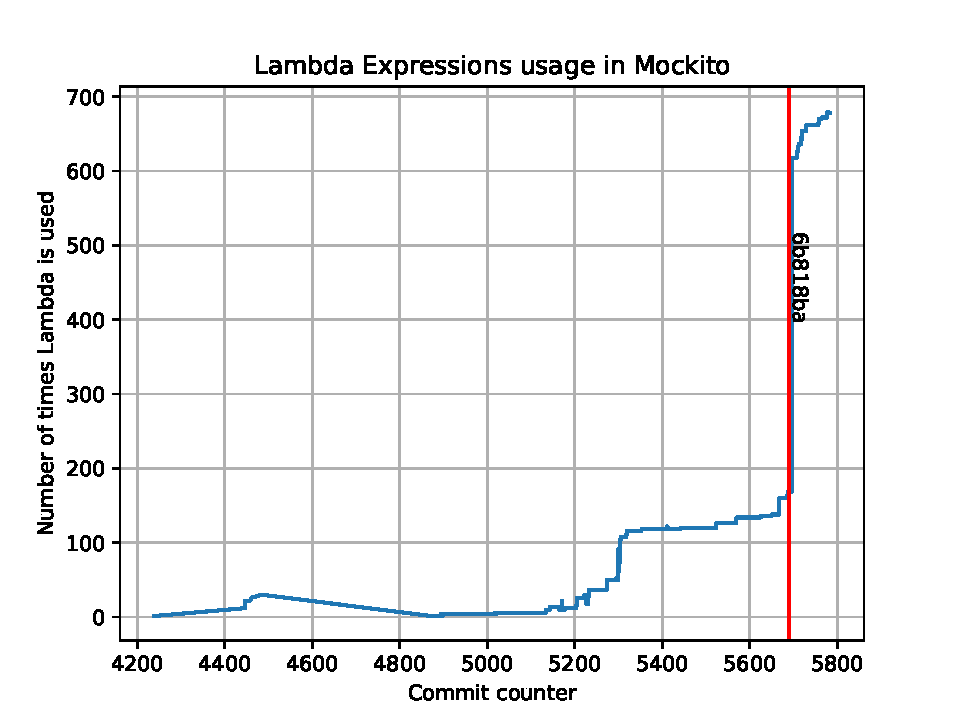
\includegraphics[width=1.\linewidth]{papers/jfeature/img/lambda_count.pdf}
\end{subfigure}%
\begin{subfigure}{.5\columnwidth}
  \centering
  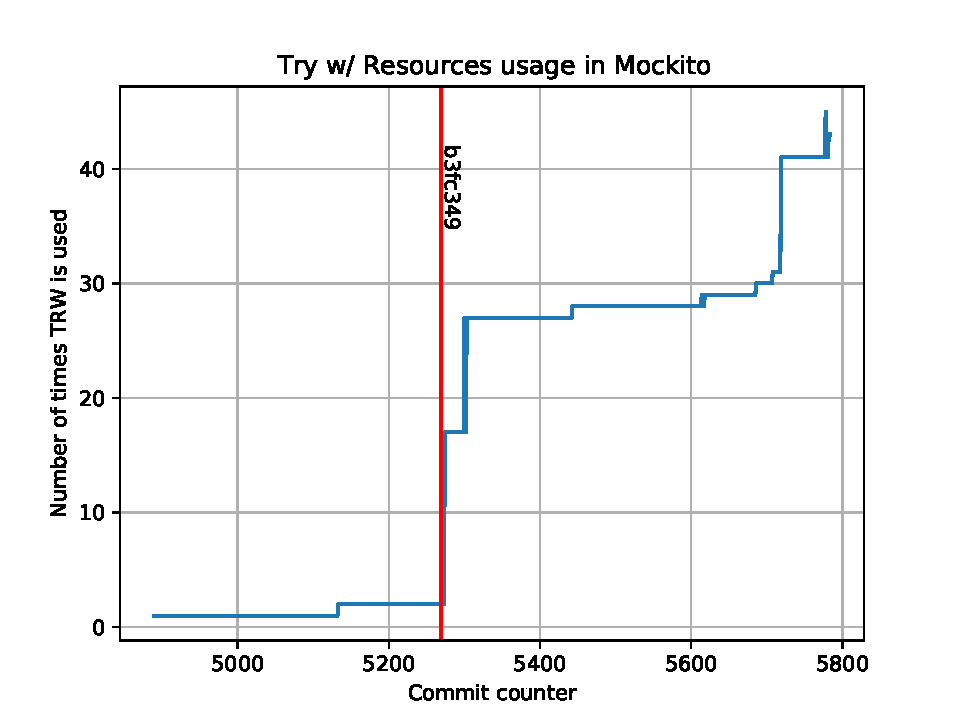
\includegraphics[width=1.\linewidth]{papers/jfeature/img/TWR_count.pdf}
\end{subfigure}%
\caption{\label{lbl:mockito} Usage of \textsc{Lambda Expressions} and \textsc{Try With Resources} in Mockito over time.}
\end{figure}
The evolution of the occurrences of \textsc{Lambda Expressions} and \textsc{Try With Resources} is depicted in Figure~\ref{lbl:mockito}. As can be seen, at commit number 5269\footnote{Commit: b3fc349.}, there is a substantial increase in utilisation of try with resources, whereas at commit number 5696\footnote{Commit: 6b818ba.}, there is a significant increase in the use of lambda expressions.

\subsection{Project mining}
Contemporary revision control hosting services (GitHub\footnote{\url{https://github.com}}, GitLab\footnote{\url{https://gitlab.com}}, bitbucket\footnote{\url{https://bitbucket.org}}) offer uniform interfaces to the source code of millions of software projects.
These interfaces enable researchers to ``mine'' software projects at scale, filtering by certain predefined properties (e.g., the number of users following the project or the main programming language).
For example, the \textit{GitHub Java Corpus}~\cite{githubCorpus2013} collects almost 15,000 projects from GitHub, filtered to only include Java projects that have been forked at least once.
Combining JFeature with these query mechanisms allows researchers to select projects by more detailed syntactic and semantic features.
For instance, a corpus suitable for answering questions about race detection~\cite{li2014rfbi}
could select projects that make explicit use of \textsc{java.util.concurrent.*},
while an exploration of functional programming patterns~\cite{cok2018reasoning} could select projects that use \textsc{Lambda Expressions} and \textsc{Method References}.
